\section{Theorie}
\label{sec:Theorie}

\subsection{Fehlerrechnung}

Für die Fehlerfortpflanzung bei Gleichungen mit $N$ fehlerbehafteten Größen
wird jeweils die Formel zur Gaußschen Fehlerfortpflanzung

\begin{equation}
  \sigma = \sqrt{\sum_{i=1}^{N}\biggl(\frac{\partial f(x_i)}{\partial x_i}
  \sigma_i\biggr)^2}
\end{equation}
mit der jeweiligen Funktion $f(x_i)$, den Messgrößen $x_i$ und den
zugehörigen Fehlern $\sigma_i$ verwendet.
Zur Berechnung des arithmetischen Mittels von $N$ Messwerten wird jeweils die
Formel

\begin{equation}
  \bar{x} = \frac{1}{N}\sum_{i=1}^{N}x_i
\end{equation}
mit den Messwerten $x_i$ benutzt.
die Standardabweichung des Mittelwerts wird jeweils mit der Gleichung

\begin{equation}
  \bar{\sigma} = \sqrt{\frac{1}{N-1}\sum_{i=1}^{N}(x_i - \bar{x})^2}
\end{equation}
mit den $N$ Messwerten $x_i$ berechnet.


\subsection{Das Prinzip einer Wärmepumpe}

Der erste Hauptsatz der Thermodynamik
besagt im Wesentlichen, dass die Energie in einem
abgeschlossenen System konstant ist. Demnach wäre es theoretisch möglich,
Wärme von einem kälteren in ein wärmeres Reservoir zu übertragen, was
erfahrungsgemäß aber nicht geschieht.
Der zweite Hauptsatz löst dieses Problem auf, denn er beinhaltet, dass diese
Übertragung nur durch Zufuhr von zusätzlicher mechanischer Energie
mittels einer Wärmepumpe möglich ist. In diesem Fall ergibt sich wegen der
Energieerhaltung die Beziehung
\begin{equation}
  Q_1 = Q_2 + A
  \label{eqn:Energieerhaltung}
\end{equation}
mit der vom wärmeren Reservoir aufgenommenen Wärmemenge $Q_1$, der vom kälteren
Reservoir abgegebenen Wärmemenge $Q_2$ und der, von der Wärmepumpe aufgewandten,
mechanischen Arbeit $A$.
Aus den Hauptsätzen folgt außerdem für die zugehörigen Temperaturen $T_1$ und
$T_2$ im Idealfall
\begin{equation}
  \frac{Q_1}{T_1} - \frac{Q_2}{T_2} = 0.
  \label{eqn:TempWaermeIdeal}
\end{equation}
Dabei wird aber davon ausgegangen, dass es sich um einen reversiblen Prozess
handelt. Gleichung \eqref{eqn:TempWaermeIdeal} gilt also nur, wenn die vom
kälteren Reservoir abgegebene Wärme $Q_2$ und die mechanische Arbeit $A$
jederzeit wieder in einem umgekehrten Prozess vollständig zurückgewonnen werden
kann. Da man praktisch nie von einem abgeschlossenen System ausgehen kann, da
beispielsweise immer ein Wärmeaustausch mit der Umgebung stattfindet, muss
Gleichung \eqref{eqn:TempWaermeIdeal} zu
\begin{equation}
  \frac{Q_1}{T_1} - \frac{Q_2}{T_2} > 0
  \label{eqn:TempWaermeReal}
\end{equation}
abgewandelt werden.
Das Verhätnis zwischen der vom wärmeren Reservoir aufgenommenen Wärmemenge $Q_1$
zwischen der geleisteten mechanischen Arbeit bezeichnet man als Güteziffer $\nu$
der Wärmepumpe. Diese gibt an, wie günstig die Wärmepumpe arbeitet, also wie
wenig Arbeitsaufwand für die Übertragung der Wärme notwendig ist.
Mit den Gleichungen \eqref{eqn:Energieerhaltung}, \eqref{eqn:TempWaermeIdeal}
und \eqref{eqn:TempWaermeReal} ergibt sich die Güteziffer einer idealen
Wärmepumpe
\begin{equation}
  \nu_\text{id} = \frac{Q_1}{A} = \frac{T_1}{T_1-T_2}
\end{equation}
und die einer realen Wärmepumpe
\begin{equation}
  \nu_\text{re} < \frac{T_1}{T_1-T_2}.
\end{equation}
An diesen Gleichungen ist erkennbar, dass eine Wärmepumpe umso günstiger
arbeitet, wenn die Temperaturdifferenz $T_1-T_2$ zwischen den beiden Reservoiren
gering ist.
Der Vorteil der Wärmegewinnung mit einer Wärmepumpe gegenüber Verfahren, in
denen mechanische Arbeit direkt in Wärme umgewandelt wird, besteht darin, dass
die gewonnene Wärmemenge $Q_1$ hierbei auch größer als die aufgewandte Arbeit
$A$ sein kann.

\subsection{Schematischer Aufbau einer Wärmepumpe}

Der schematische Aufbau einer Wärmepumpe ist in Abbildung
\ref{fig:WaermepumpeSchematisch} dargestellt.
Die Wärme wird über die Verdampfungswärme eines realen Gases mit
hoher Kondensationswärme übertragen. Dabei nimmt das Gas am kühleren
Reservoir mit der Temperatur $T_2$ bei kleinem Druck $p_\text{a}$ die
Verdampfungswärme
$L$ auf und verdampft. Dann strömt es in den Kompressor $K$, in welchem es nahezu
adiabatisch, also ohne Wärmeverluste, komprimiert wird und somit weitere Energie
aufnimmt.
Von dort aus gelangt das Gas in das zweite Reservoir mit der Temperatur $T_1$,
in welchem es dann bei
höherem Druck $p_\text{b}$ die aufgenommene Verdampfungswärme $L$ abgibt und
kondensiert. Zuletzt strömt die Flüssigkeit durch einen Reiniger, der
Gasblasen entfernt, und durch ein Drosselventil, an welchem der Druckunterschied
aufrecht erhalten wird, zum ersten Reservoir.
Der Kreislauf des Stoffes wird durch den Kompressor, also das Bauteil, welches
die für eine Wärmeübertragung nötige, mechanische Arbeit verrichtet,
gewährleistet.

\begin{figure}
  \centering
  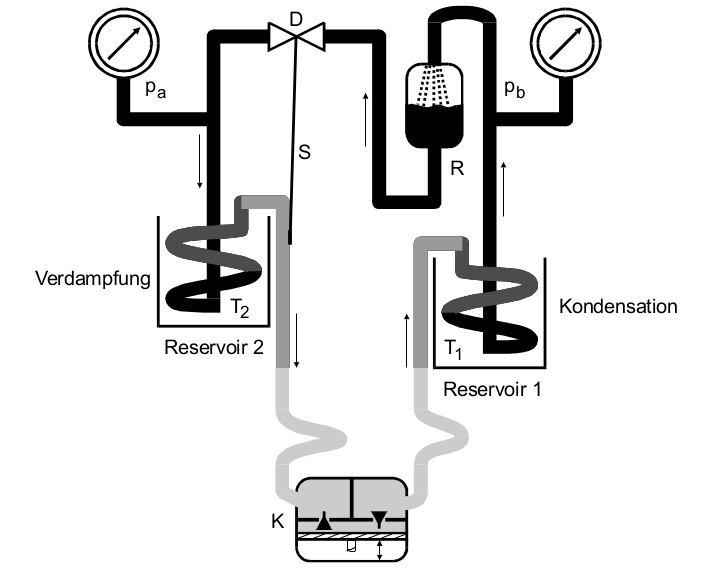
\includegraphics[height = 8cm]{WaermepumpeSchematisch.png}
  \caption{Schematischer Aufbau einer Wärmepumpe. $p_\text{b} > p_\text{a}$,
  $T_1 > T_2$ \cite{anleitung}}
  \label{fig:WaermepumpeSchematisch}
\end{figure}

\subsection{Kenngrößen einer realen Wärmepumpe}


\subsubsection{Bestimmung der realen Güteziffer}

Die pro Zeiteinheit gewonnene Wärmemenge $\frac{\increment Q_1}{\increment t}$ im
wärmeren Reservoir lässt
sich mit der Gleichung
\begin{equation}
  \frac{\increment Q_1}{\increment t} = (m_1 c_\text{w} + m_\text{k}c_\text{k})
  \frac{\increment T_1}{\increment t}
\end{equation}
berechnen, wobei $m_1 c_\text{w}$ und $m_\text{k}c_\text{k}$ die
Wärmekapazitäten des Wassers und der Kupferschlange und des Eimers im wärmeren
Reservoir sind und der Quotient $\frac{\increment T_1}{\increment t}$ die
dort gewonnene Temperatur pro Zeiteinheit.
Mit der über den gesamten Zeitraum gemittelten Leistung $\bar{N}$ des
Kompressors folgt für die reale Güteziffer der Wärmepumpe
\begin{equation}
  \nu = \frac{1}{\bar{N}}\frac{\increment Q_1}{\increment t}.
\end{equation}

\subsubsection{Bestimmung des Massendurchsatzes}

Die pro Zeiteinheit verlorene Wärmemenge $\frac{\increment Q_2}{\increment t}$ im
kälteren Reservoir lässt sich mit der Gleichung
\begin{equation}
  \frac{\increment Q_2}{\increment t} = (m_2 c_\text{w} + m_\text{k}c_\text{k})
  \frac{\increment T_2}{\increment t}
\end{equation}
berechnen, wobei $m_2 c_\text{w} + m_\text{k}c_\text{k}$ die entsprechenden
Kapazitäten sind und $\frac{\increment T_2}{\increment t}$ die Abkühlung pro Zeiteinheit
ist.
Ist die Verdampfungswärme $L$ gegeben, so kann der Massendurchsatz mit
\begin{equation}
  \frac{\increment m}{\increment t} = \frac{1}{L}\frac{\increment Q_2}{\increment t}
\end{equation}
bestimmt werden.

\subsubsection{Bestimmung der Kompressorleistung}

Mit der Poissonschen Gleichung
\begin{equation}
  p_\text{a}V_\text{a}^\kappa = p_\text{b}V_\text{b}^\kappa = pV^\kappa,
  \label{eqn:Poisson}
\end{equation}
wobei $\kappa$ das Verhältis der Molwärmen $C_p$ und $C_V$ ist,
folgt für die Arbeit, die der Kompressor leistet, wenn er ein Gasvolumen von
$V_\text{a}$ auf $V_\text{b}$ verringert,
\begin{equation}
  A_\text{m} = - \int_{V_\text{a}}^{V_\text{b}} p \symup{d}V =
  \frac{1}{\kappa - 1} \Bigl(p_\text{b} \sqrt[\kappa]{\frac{p_\text{a}}
  {p_\text{b}}} - p_\text{a} \Bigr) V_\text{a}.
\end{equation}
Daraus ergibt sich die Kompressorleistung
\begin{equation}
  N_\text{mech} = \frac{\increment A_\text{m}}{\increment t} =
  \frac{1}{\kappa - 1} \Bigl(p_\text{b} \sqrt[\kappa]{\frac{p_\text{a}}
  {p_\text{b}}} - p_\text{a} \Bigr) \frac{1}{\rho} \frac{\increment m}
  {\increment t}
\end{equation}
mit der Dichte des Transportmediums $\rho$.
